\section{Algoritme til detektering af gang, løb og cykling}
\textit{I dette afsnit udarbejdes en algoritme som har til formål at adskille aktiviteterne gang, løb og cykling... }

\subsection{Design}
For at kunne adskille gang, løb og cykling benyttes et accelerometer og et gyroskop som er beskrevet i \secref{LSM9DS1}\fxnote{opg: tjek op på denne reference}. Herunder vil gyroskopet blive benyttet til at detektere cykling, mens løb og gang detekteres ved brug af accelerometeret. For at kunne detektere og adskille disse aktiviteter, behandles inputtet fra sensorerne gennem forskellig signalbehandling, hvorefter algoritmer afgør om de pågældende signaler repræsenterer gang, løb, cykling eller ingen aktivitet. 

\subsubsection{Algoritme til gang og løb}
Data fra accelerometerets y-akse skal signalbehandles, førend en algoritme kan detektere og adskille gang fra løb. Måden hvorpå dataet vil blive behandlet er først ved at fjerne støj ved brug af et elliptisk filter. Dette skal være et 4. ordens lavpas elliptisk filter med et pasbånd fra 20 til 100 Hz, og med en dæmpningsgrad på 60 dB\fxnote{og 0.5 dB peak-to-peak ripples}. Efterfølgende divideres det filtrerede signal med 8 og kvadreres. Resultatet heraf betyder at signaler som ikke relaterer sig til hælnedslaget minimeres kraftigt, og selve hælnedslaget forstærkes.\fxnote{ved gang er det swing og heel strike, ved løb er det primært kun heel strike, men også lidt toe offset.}
Afslutningsvis vil signalet blive filtreret med et moving average filter som udglatter signalet, hvilket resulterer i at små udslag i signalet ikke opfattes, og signalets hælnedslag vil fremstå tydeligere. \\
Resultatet af ovenstående signalbehandling medfører at der findes et udtryk for gang og løbs amplitude forhold. Ud fra denne behandling af pilotforsøgets data vurderes det, at amplituden for hælnedslag ved løb er over 0,65 og ved gang er over 0,04, hvorfor signaler med amplituder under 0,04 ikke vurderes som værende aktivitet.
\begin{figure}[H]
	\centering
	\includegraphics[scale=0.5]{figures/cDesign/algoritme_gl.png}
	\caption{Flowchart over algoritmen til detektering af gang og løb}
	\label{fig:algoritme}
\end{figure}
Ovenstående figur repræsenterer algoritmen for detektering og adskilles af gang og løb. Førend algoritmen tilhørende gang og løb starter, undersøges hvorvidt cykling registreres. Hvis dette ikke er tilfældet og løb detekteres skal en counter starte og først stoppe når løb ikke længere detekteres. Når counteren stopper gemmes varigheden for counteren i et array tilhørende udført løb. Hvis løb ikke detekteres, undersøges der hvorvidt gang registreres. Hvis gang registreres skal en counter starte og først stoppe når gang ikke længere detekteres. Når counteren stopper gemmes varigheden for counteren i et array tilhørende udført gang. Hvis algoritmen for detektering af løb og gang ikke registrer aktiviteterne, så bliver der ikke udført nogen bevægelse, og algoritmen starter forfra.

\subsection{Cykling}
Data fra gyroskopets z-akse skal signalbehandles, førend en algoritme kan detektere og adskille aktiviteterne. Første step i denne signalbehandling er at udføre en Fast Fourier Transform (FFT) over fire sekunders sampling. Dette medfører at signalets magnitude og dets tilhørende frekvenser kommer til udtryk, hvoraf andet step indledes. Dette step finder den maksimale magnitude med tilhørende frekvens. Tredje step består af to summeringer, første summering summerer FFT'en fra den frekvens hvor den største magnitude befandt sig $\pm 1$Hz. Anden summering summerer FFT'en fra 1 til 20 Hz. Disse integraler indleder fjerde og sidste step, som omregner hvor stor en procentdel første integrale udgør af signalets totale energi. \\
Resultatet af ovenstående signalbehandling medfører at der opstilles et udtryk for signalets spredning af energi. Det gør sig gældende at cykling har en spredning af energi fordelt nært frekvensen med den største amplitude. Data fra gyroskopets z-akse vedrørende cykling blev for alle forsøgspersoner, behandlet med ovenstående metode. Dette resulterede i at 84,5\% til 91,9\% af energien lå $\pm 1$Hz omkring den fundne frekvens. Følgende blev ligeledes behandlet for gang og løb, for at sikre disse ikke havde samme spredning i frekvensområdet, hvormed en mulig tærskelværdi til detektering af cykling, kan fastsættes.  Dette resulterede i at ved gang befandt energien omkring den fundne frekvens sig mellem 35,9\% til 48,5\% og ved løb befandt energien omkring den fundne frekvens sig mellem 42,8\% til 60,5\%. \\
Resultatet af at energien omkring den fundne frekvens med den største amplitude er $\approx$30\% større ved cykling end ved gang og løb, fastsættes tærskelværdien til 70\%. For at detektere cykling skal outputtet fra databehandlingen være større end 70\%.

\begin{figure}[H]
	\centering
	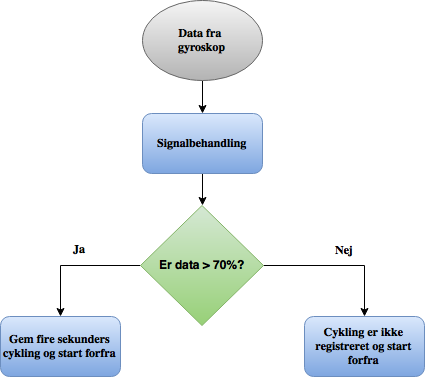
\includegraphics[scale=0.6]{figures/cDesign/algoritme_cykling.png}
	\caption{På figuren ses et flowchart som gennemgår algoritmen vedrørende detektering af cykling.}
	\label{fig:algoritme_cykling}
\end{figure}

Ovenstående figur repræsenterer algoritmen for detektering af cykling. Hvis cykling detekteres skal en counter starte og først stoppe når cykling ikke længere detekteres. Når counteren stopper gemmes varigheden af counteren i et array tilhørende udført cykling. Hvis cykling ikke detekteres skal gyroskopet gå i LPM i 10 sekunder før algoritmen køres igen. 






\subsection{Implementering}




\subsection{Test}


